\documentclass[12pt]{article}
\usepackage{graphicx} % Required for inserting images
\usepackage{wrapfig}
\usepackage{amsmath}
\usepackage{amssymb}
\usepackage{dsfont}
\usepackage[margin=1in]{geometry}


\title{\vspace{-4em}Problem Set 1}
\author{Cem Kozanoglu \\ Collaborators: Wooyong Park, Roberto Telles-Gonzalez}
\date{September 2025}

\begin{document}

\maketitle

This document describes and explains the results that were obtained from the code in pset1.ipynb. The code was written in Python using the Polars library for data manipulation and analysis, and Matplotlib for visualization.

\section{Question 1}

\subsection{Part A}

The first test statistic we use is the difference in means between the treatment and control groups, described by $T_1$ in formula:

\[T_1 = \bar{Y}_T - \bar{Y}_C\]

I generated 100,000 simulations of the test statistic under the null hypothesis of no treatment effect. The histogram below shows the distribution of the simulated test statistics, with a red dashed line indicating the observed test statistic from the actual data.

\vspace*{2em}
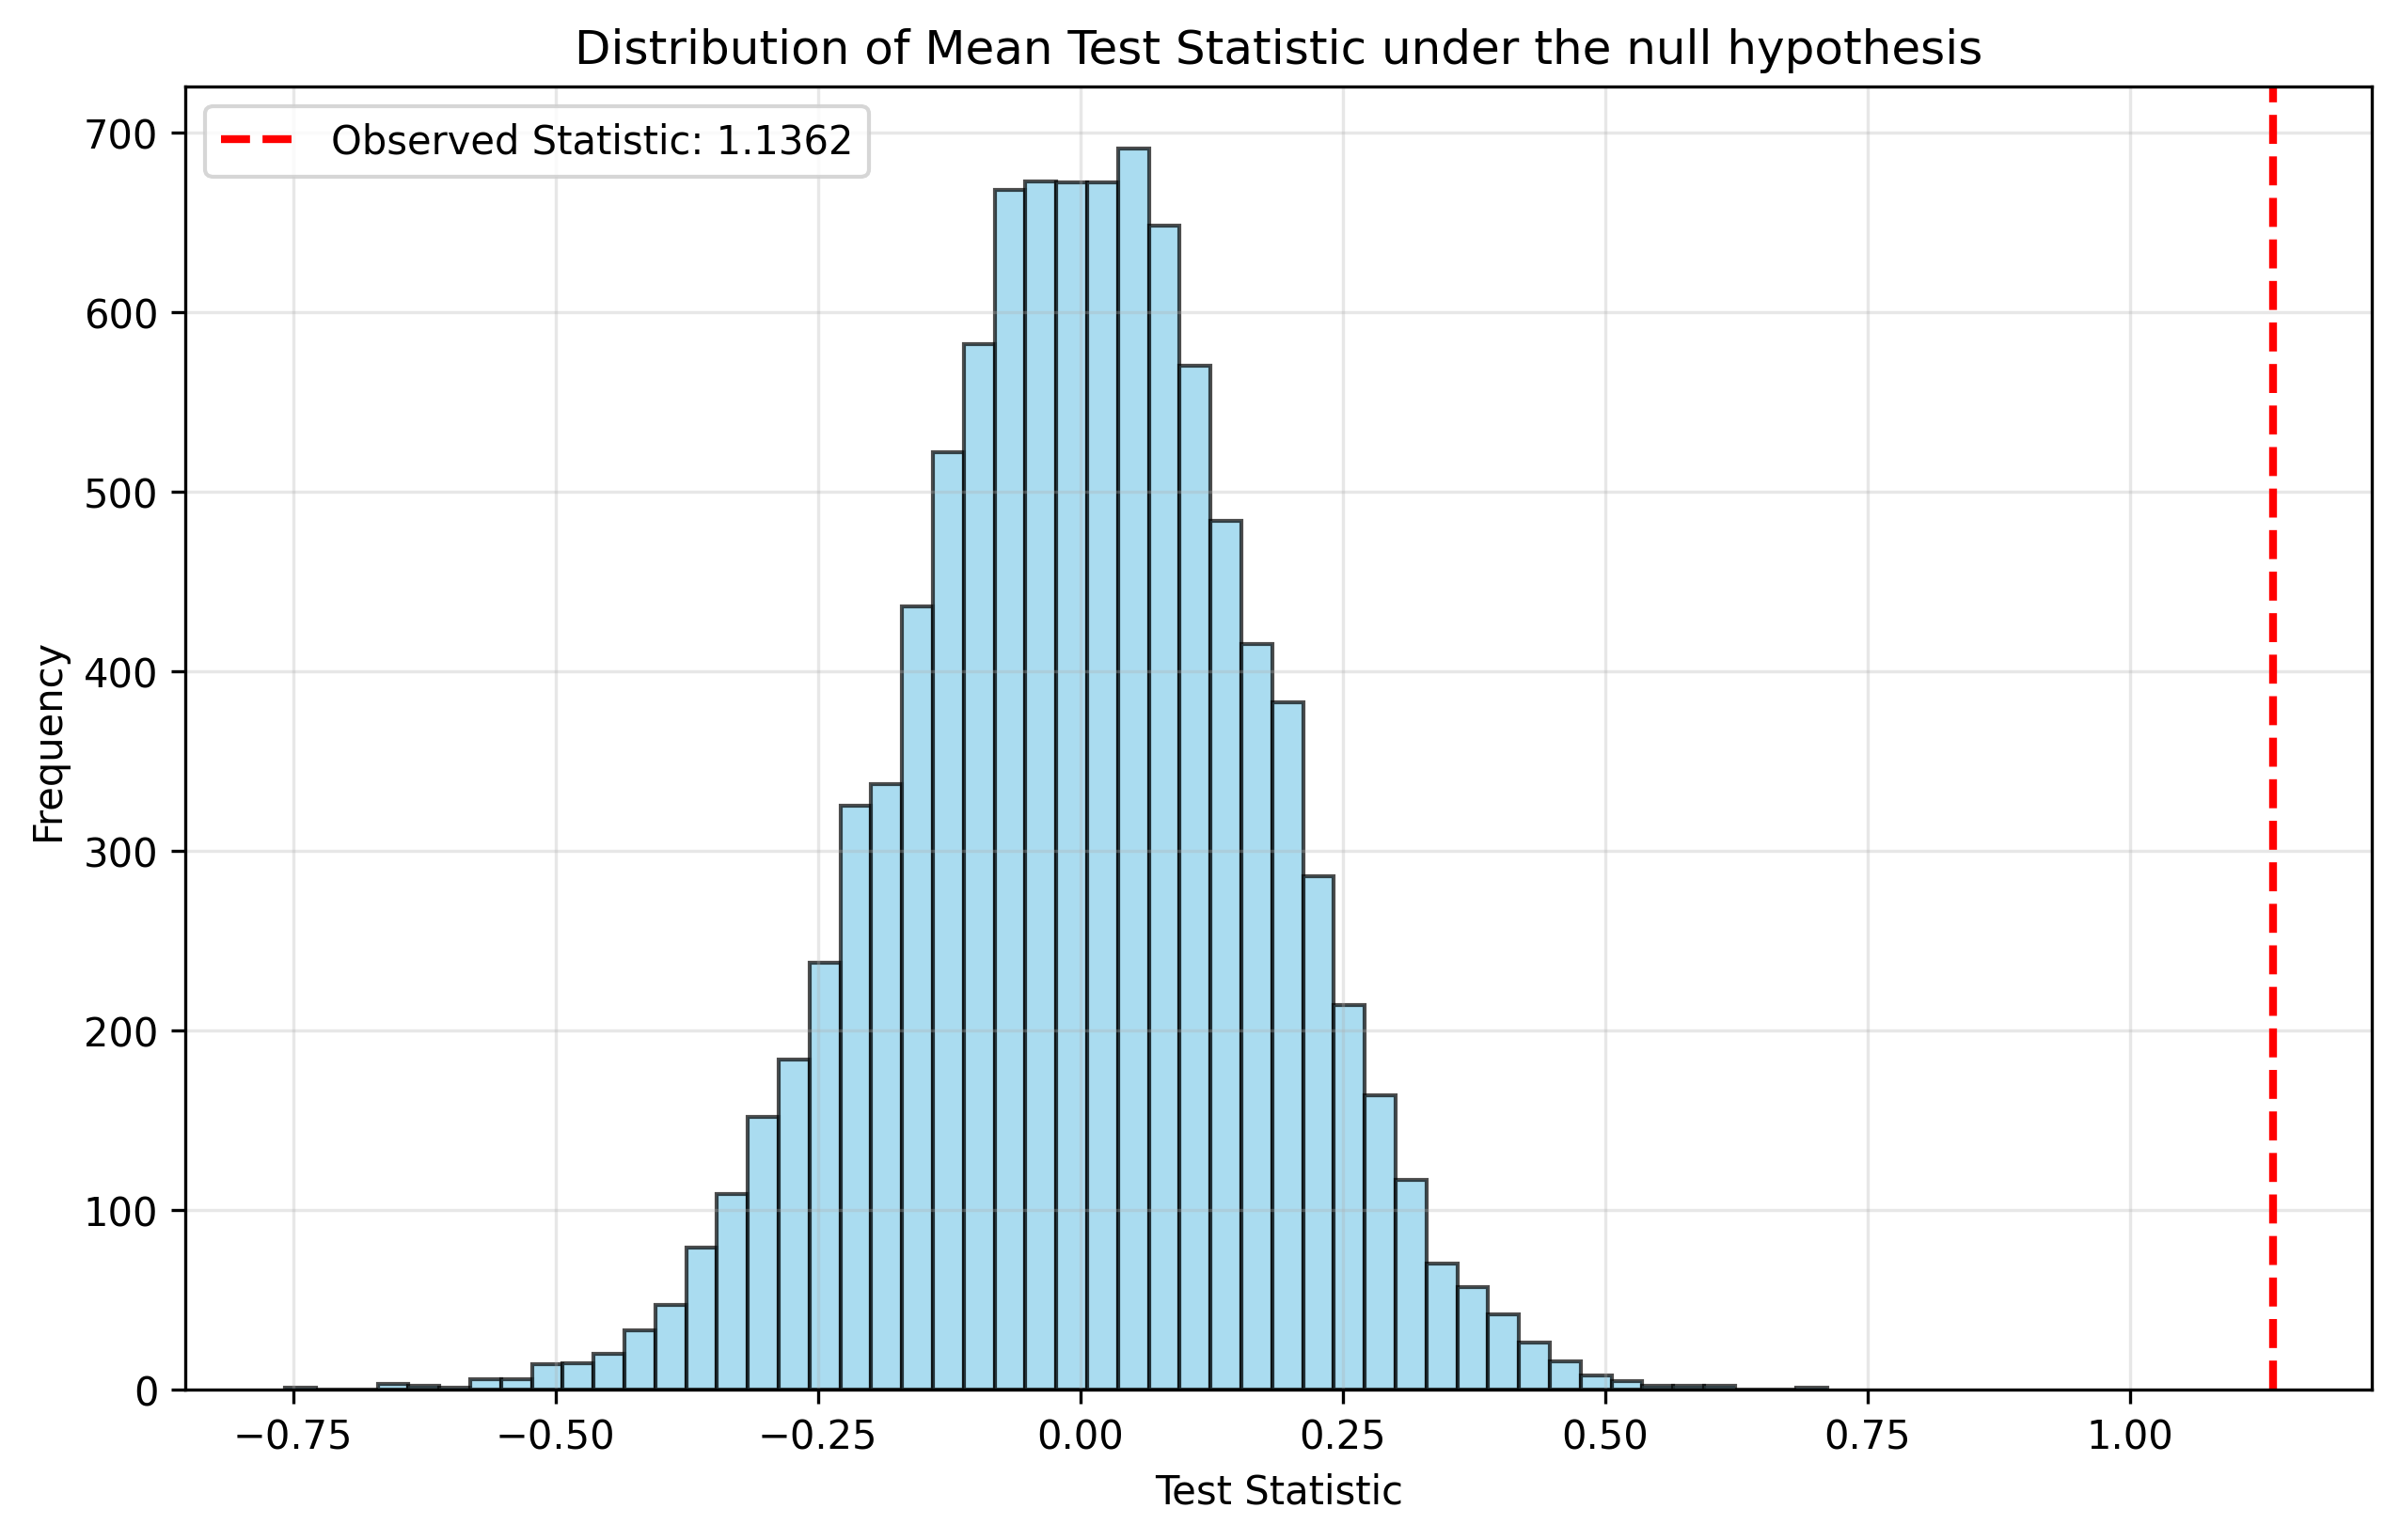
\includegraphics[width=0.8\textwidth]{stat1_graph.png}
\vspace*{2em}

While the trials converged to a normal distribution around 0 (as we might have expected), our observed T-statistic was 1.1362, extremely unlikely given the null hypothesis. The exact p-value for the observed statistic was 0.00, meaning that there were literally no datapoints in any of our simulations which were as extreme or more extreme than our observed test statistic. This suggests that the treatment had a statistically significant effect on earnings reported after one year.

\subsection{Part B}

In most cases the difference in means will be the most important statistic to consider when trying to grasp the effects of a treatment. However there may be cases where the mean is not the best measure of central tendency, such as when there are significant outliers in the data, in which case the median may be a more appropriate measure to consider. On the other-hand, one issue which afflicts tests based on medians is 'zero-inflation', where a large number of observations with value zero can mean that the median is likely to be zero for both treatment and control and unlikely to be informative. 
\newline


My prior is that the treatment is likely to have a similar effect for most individuals, and the empirical data is indeed zero-inflated which means that we should be careful when considering the difference-in-medians test statistic as it may not be telling us much about the data.
\newline

With these disclaimers, we can go ahead and calculate the second test statistic as the difference in medians between the treatment and control groups, described by $T_2$ in formula:

\[T_2 = \tilde{Y}_T - \tilde{Y}_C\]

I also calculated this statistic for 100,000 simulations under the null hypothesis of no treatment effect. The histogram below shows the distribution of the simulated test statistics, with a red dashed line indicating the observed test statistic from the actual data.

\vspace*{2em}
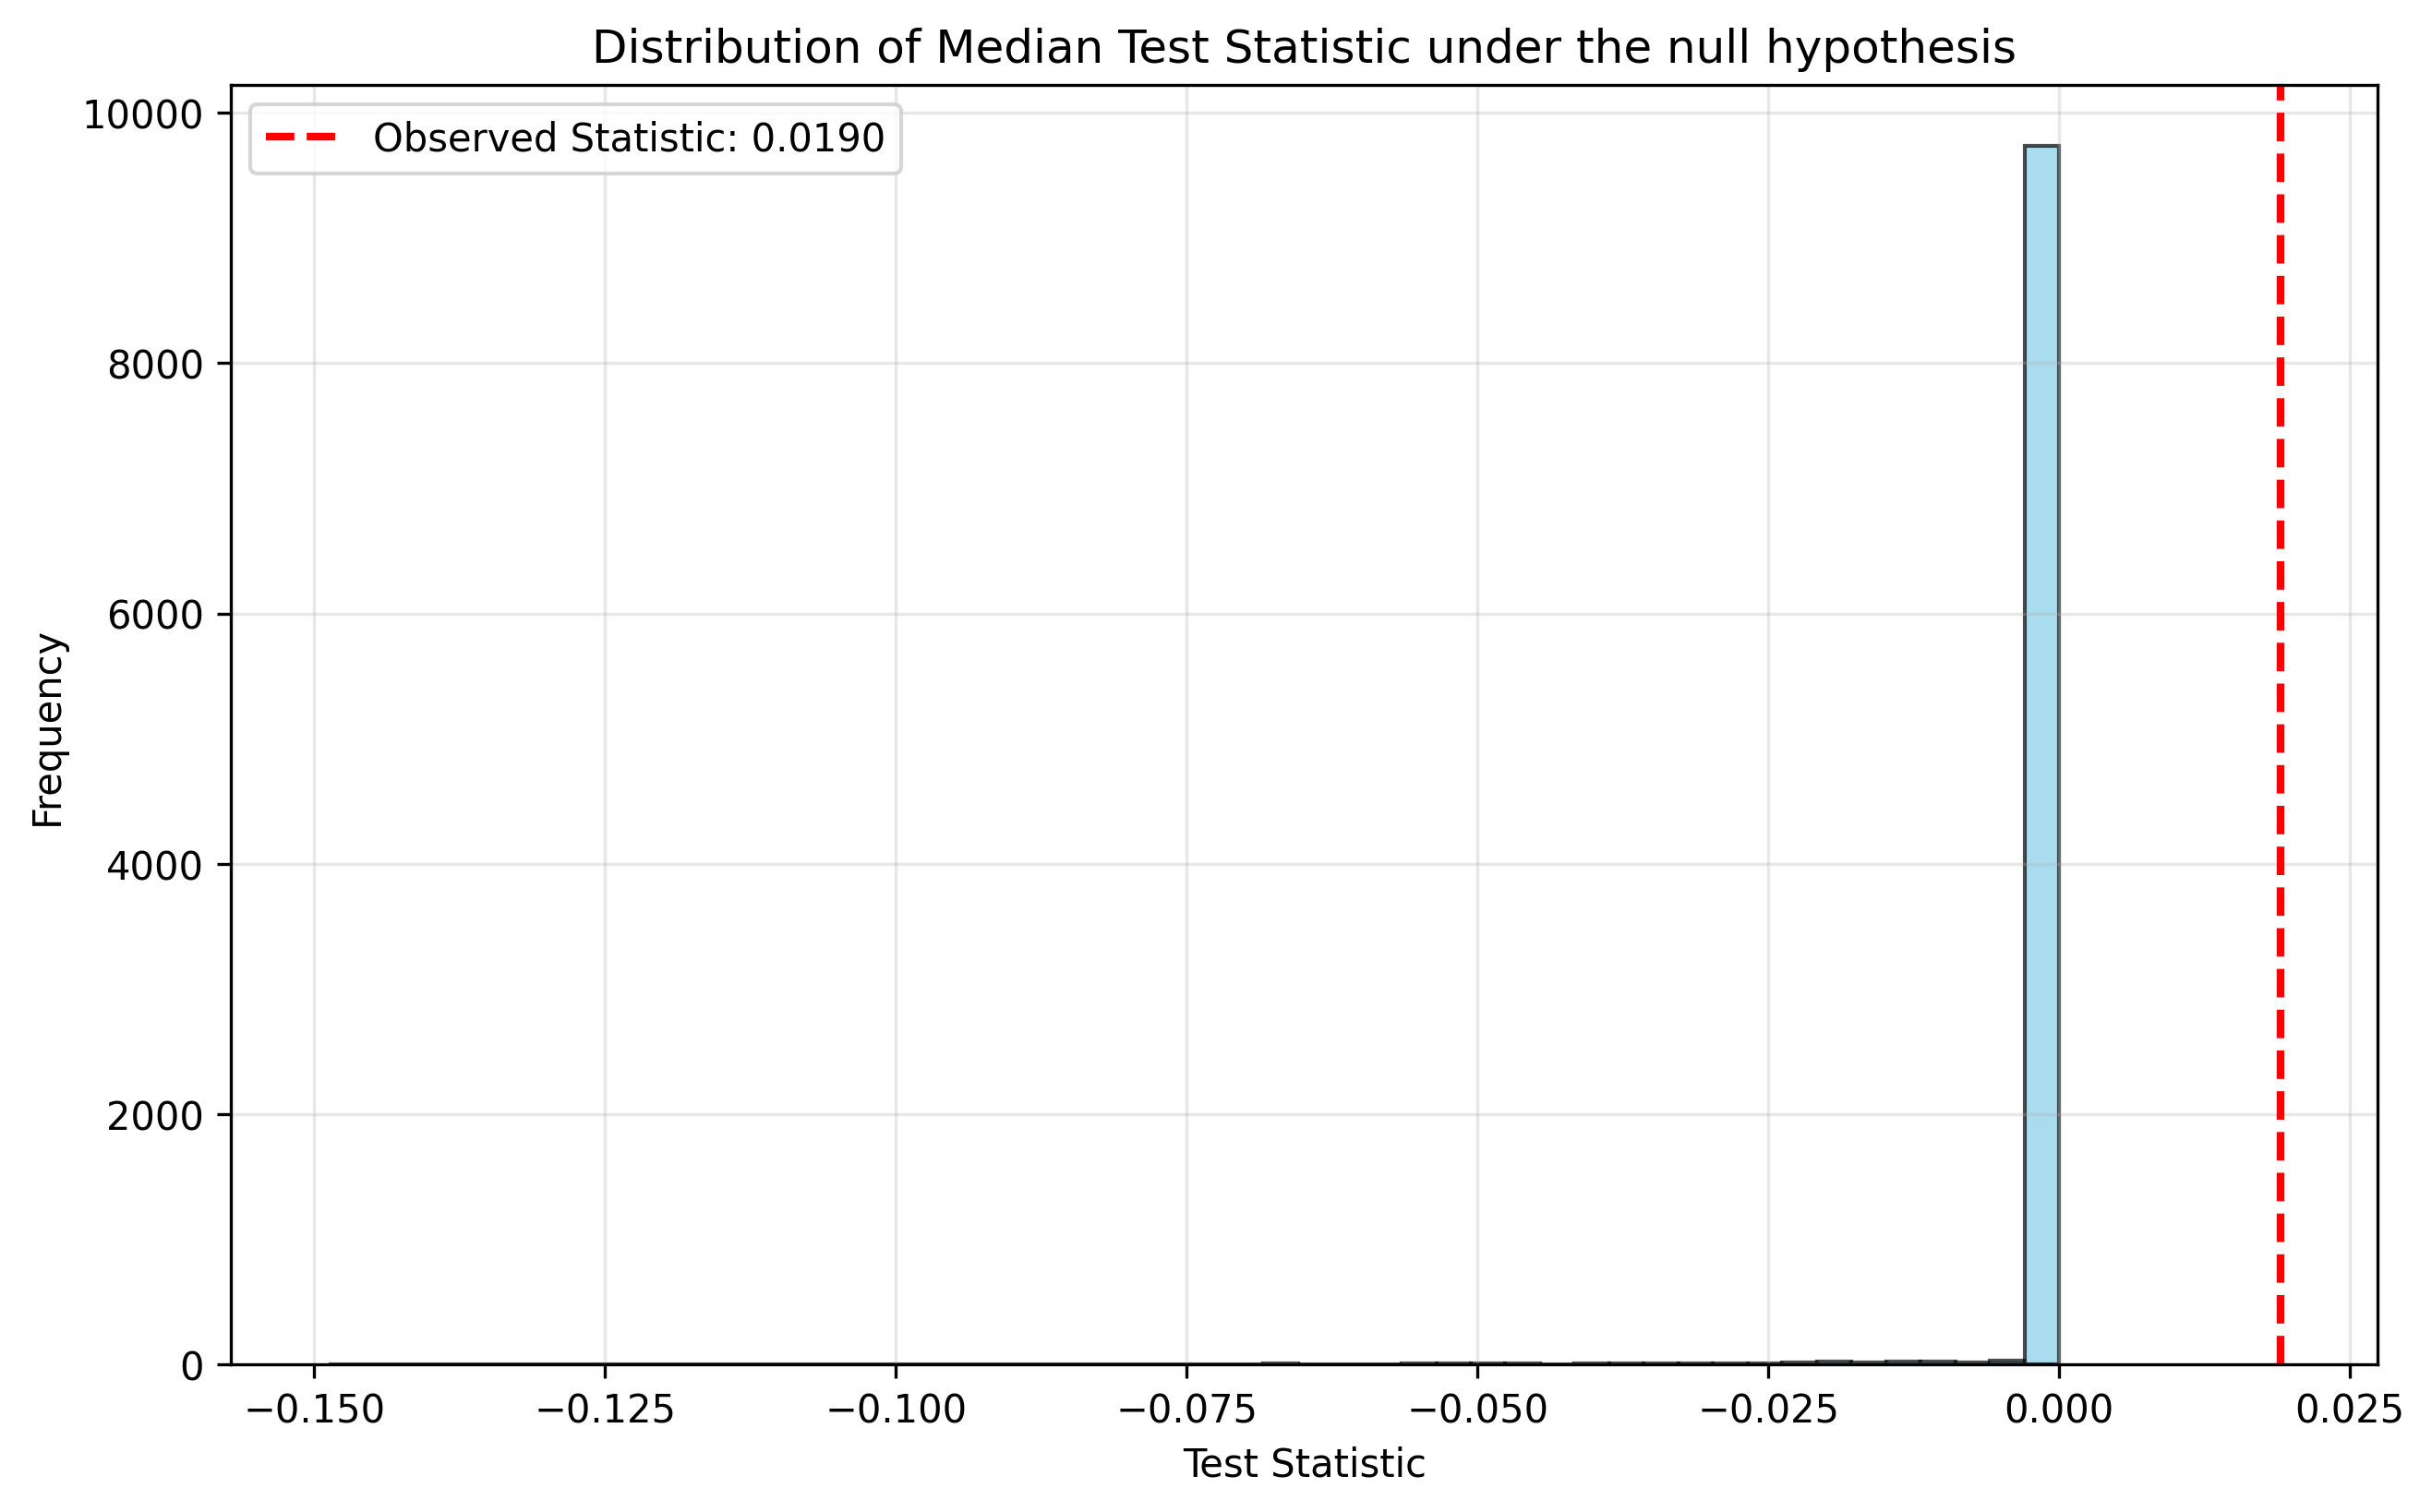
\includegraphics[width=0.8\textwidth]{stat2_graph.png}
\vspace*{2em}

The trials are clustered tightly around 0 which makes sense given that the median is less sensitive to outliers and our high sample size. Our observed statistic was 0.019, which is again very unlikely under the null hypothesis, and the exact p-value was 0.02, meaning that only 2\% of our simulated test statistics were as extreme or more extreme than our observed statistic. While less extreme than the first statistic, this again suggests that the treatment had a statistically significant effect on earnings reported after one year.


\subsection{Part C}

To further understand the effects of the treatment, we can also look at the ratio of the variances of the treatment and control groups, 
\newline

This third test statistic is described by $T_3$ in formula:

\[T_3 = S^2_T / S^2_C\]

where:

\[S^2 = \frac{1}{n-1} \sum_{i=1}^{n} (Y_i - \bar{Y})^2\]

I calculated this statistic for 100,000 simulations under the null hypothesis of no treatment effect. The histogram below shows the distribution of the simulated test statistics, with a red dashed line indicating the observed test statistic from the actual data.

\vspace*{2em}
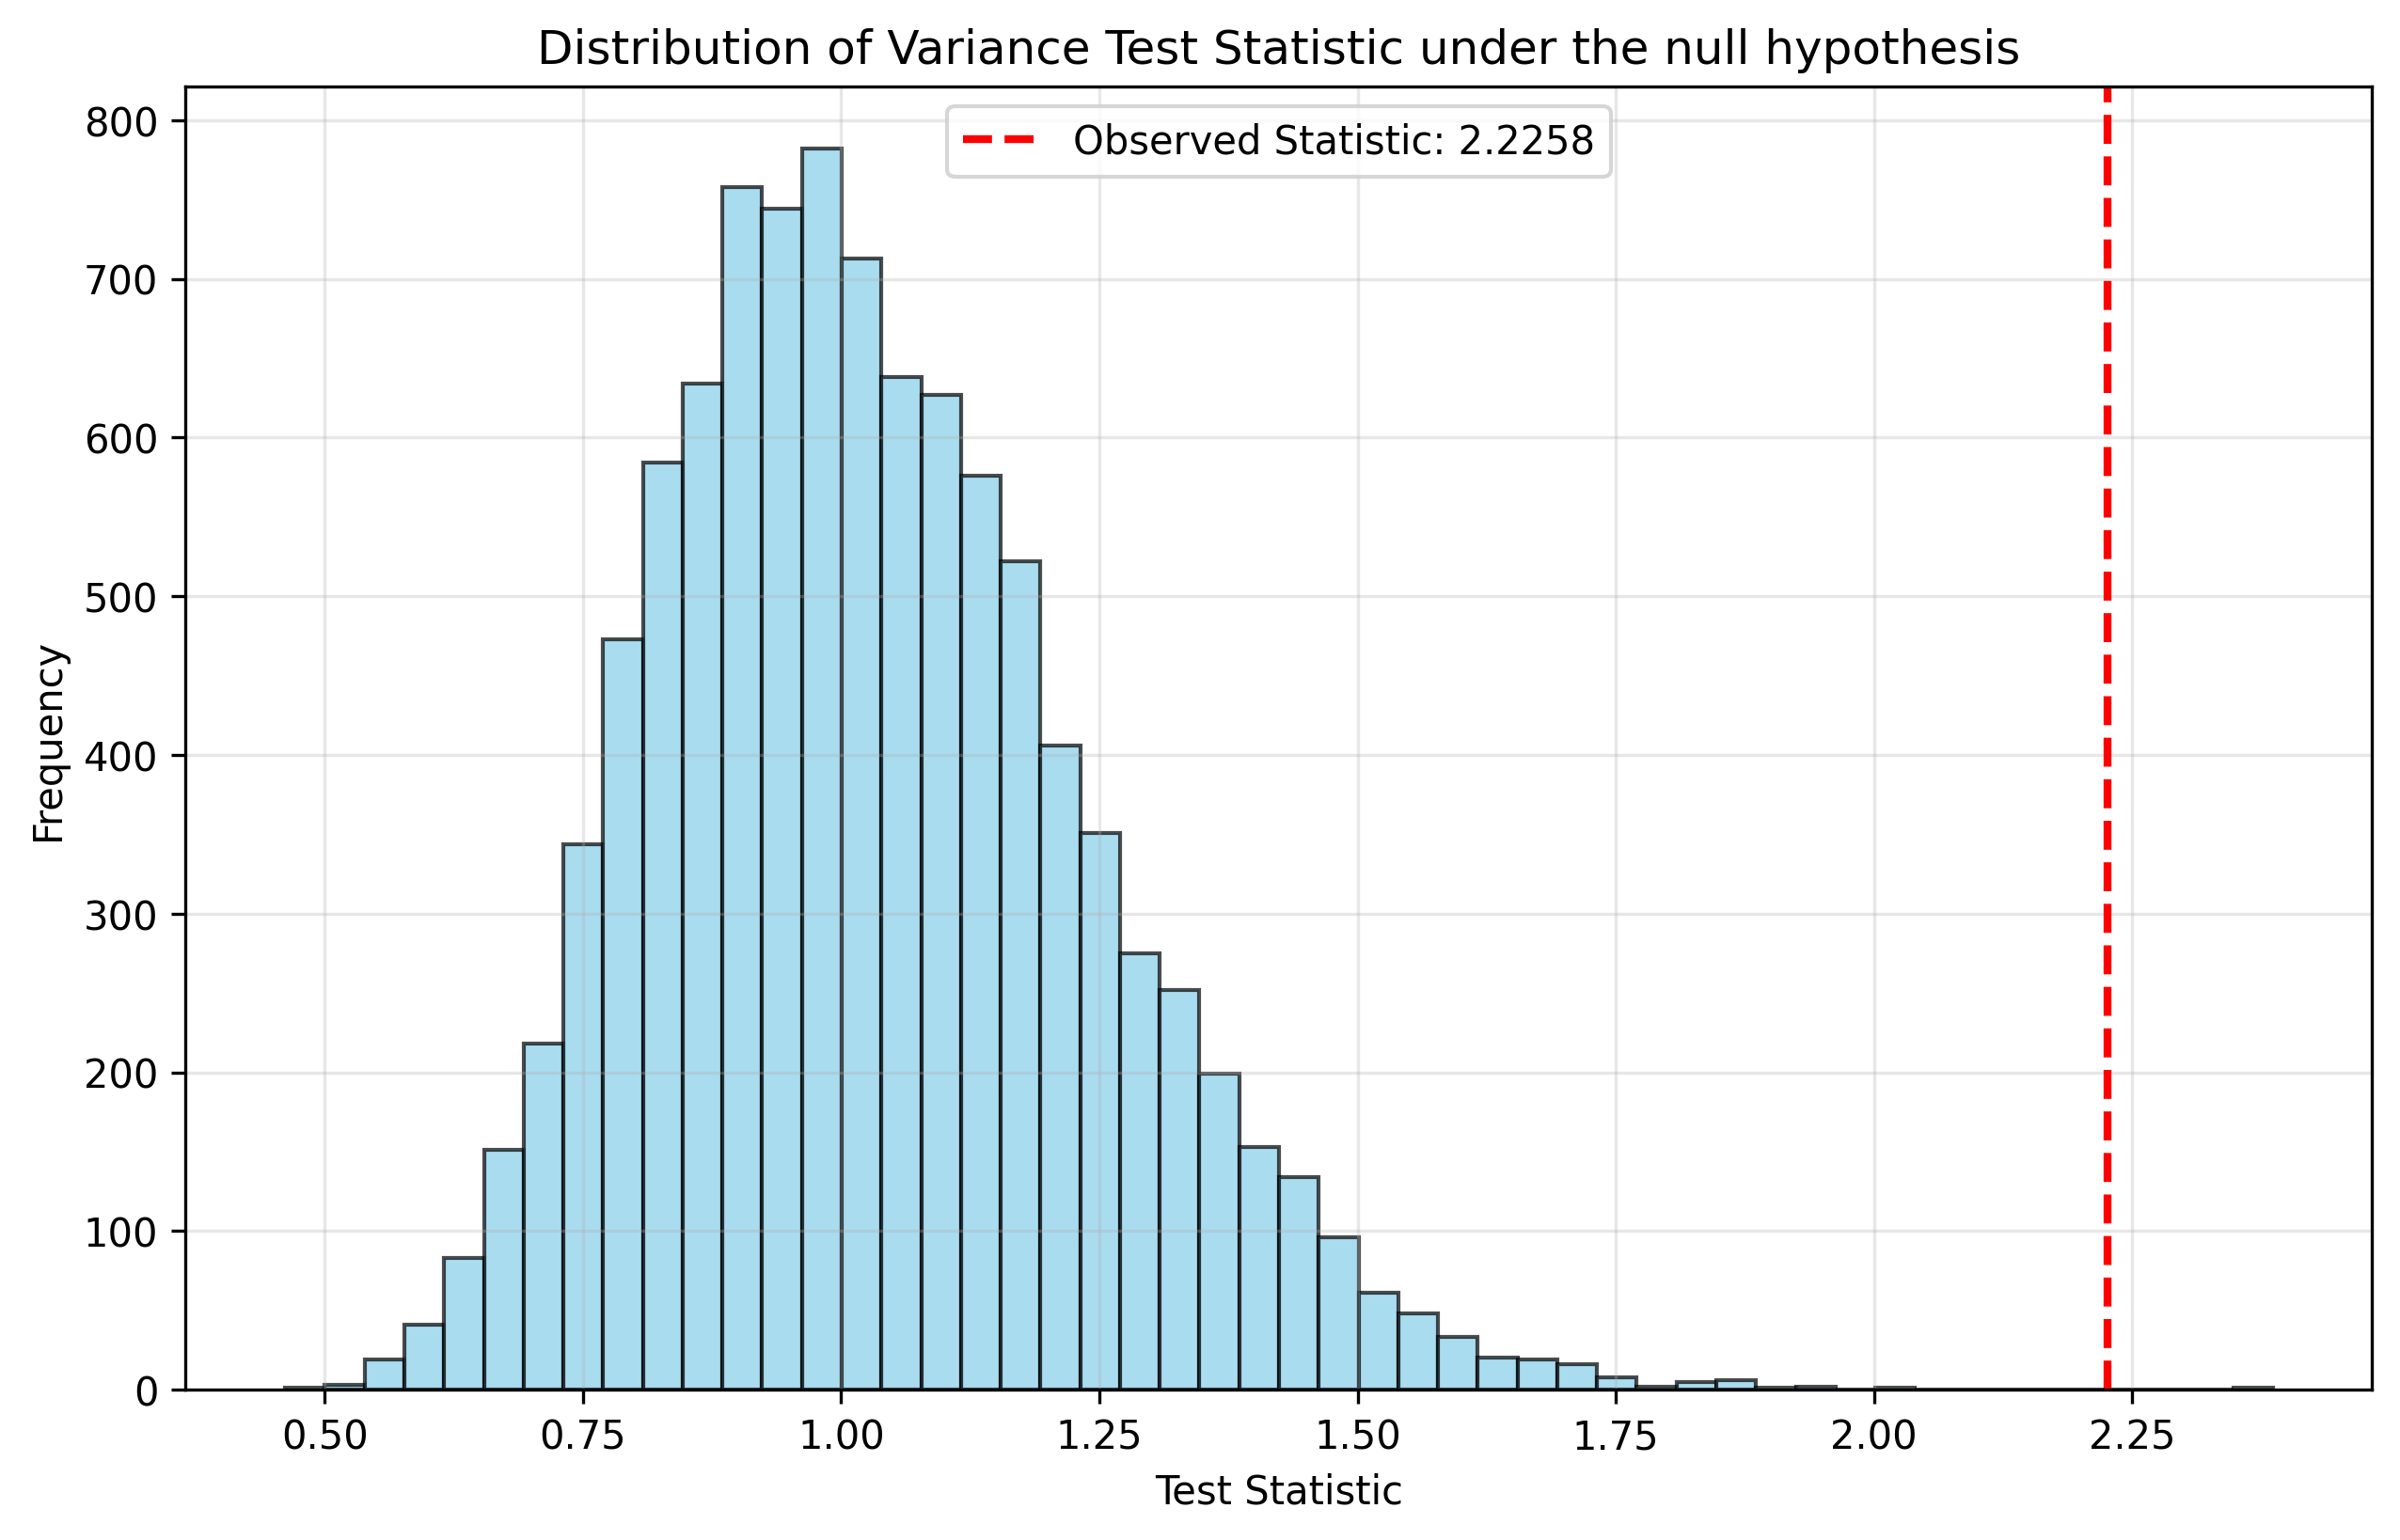
\includegraphics[width=0.8\textwidth]{stat3_graph.png}
\vspace*{2em}

In line with our findings for the last two statistics, the trials are clustered tightly around 0. Our observed statistic was 14.97, which is again very unlikely under the null hypothesis, and the exact p-value was 0.03. This again suggests that the treatment had a statistically significant effect on earnings reported after one year, and specifically that it increased the variance of earnings in the treatment group relative to the control group. This could suggest that while the treatment was beneficial on average, it may have had more varied effects on different individuals, potentially benefiting some significantly while having little to no effect on others.

\subsection{Part D}

For this section we assign the treatment randomly by using a bernoulli random variable with p = 0.2 to determine wheter a given row will be recorded as a treated or control observation. 
\newline

The findings from this random assignment are shown in the table below:

\begin{center}
\begin{tabular}{|c | c | c |} 
 \hline
 Statistic & Combinatoric p-value & Randomized p-value  \\ [0.5ex] 
 \hline
 $T_1$ & 0 & 0  \\ [0.5ex]
 \hline
 $T_2$ & 0.01641 & 0.01403  \\ [0.5ex]
 \hline
 $T_3$ & 0 & 0.00001 \\ [0.5ex] 
 \hline
\end{tabular}
\end{center}


As can be seen, our results differ very little from the original combinatoric assignment. This is likely because the high sample size of 5419 is large enough that the random assignment converges to the combinatoric assignment thanks to the Central Limit Theorem.

This type of randomisation would not be ideal in cases with a low sample size, or a low treatment probability, as it would be way more sensitive to variation. For our purposes getting 1000 or 1200 treatment observations does not make a large difference, but if p=0.01 and our number of observations varied from 40 to 60 that would likely have a significant effect on our results.

\section{Part 2}

The choice between combinatoric (fixed count) and random (bernoulli) assignment mechanisms can have meaningful implications for the analysis of experimental data, especially when our sample size is low. The difference between the random and fixed approach depends on the balance in size between the treatment and control groups, as well as the overall size of our sample size. An exposition is presented below:
\newline

We begin with the fact that the variance of our test statistic is proportional to $\frac{1}{n_t} + \frac{1}{n_c}$, where $n_t$ and $n_c$ are the sizes of the treatment and control groups respectively. This means that for a fixed total sample size n, the variance of our test statistic is minimized when $n_t = n_c$.
\newline

Now if we let $n_t = m$ where m is the actual treatment size, and $f:= n_t/n$, the proportion of treated observations, we can see that the variance of our test statistic is proportional to $\frac{1}{f(1-f)}$. 
\newline

Whereas if we let $n_t$ be a random variable with $n_t \sim Binom(n,p)$, we have our variance proportional to $E\left[\frac{1}{n_t} + \frac{1}{n_c}\right] > \frac{1}{E[n_t]} + \frac{1}{E[n_c]} = \frac{1}{np} + \frac{1}{n(1-p)} = \frac{1}{n p (1-p)}$ according to Jensen's inequality.
\newline

For large n, this difference between the expected variance and the actual (the first inequality) will be miniscule, so the greater part of the difference derives from whether our random distribution is more balanced (p closer to 0.5) than our fixed distribution (f).
\newline

In this case $p(1-p)/f(1-f) = 0.5^2/(0.49*0.51) \approx 1.0004$, meaning that our random assignment mechanism has a variance that is only 0.04\% lower than our fixed assignment mechanism, which is negligible.
\newline

However once we account for the Jensen's inequality term which makes the variance of the random assignment slightly larger, it is in fact likely that our random assignment mechanism has a slightly higher variance overall, yet still by a negligible amount.

To sum up, while the choice between combinatoric and random assignment mechanisms can have meaningful implications for the analysis of experimental data, especially when our sample size is low or our distribution is unbalanced, in this case the difference is negligible either way.

\end{document}
